\chapter{Evaluation}
% take a step back and put your results from 4 into context. 
This chapter critically examines the machine learning models conceived and partially implemented
in the previous chapter.
Table~\ref{tab:evaluation_criteria} shows an overview of the evaluated criteria. These are
structured according to the Goal-Question-Metric approach.

The quality metrics are oriented on the quality model from
\cite[]{siebert2022construction}, which is based on the ISO/IEC 9126 standard for the
evaluation of software quality. The standard was changed to fit the requirements of machine
learning models~\cite{siebert2022construction}.

The metrics of the goal \textit{Robustness} where original only defined for classification models
and therefore needed to be changed.
\textit{TODO: Explain what has been changed}

\captionsetup{margin={5pt,5pt}}

\begin{table}[H]
    \begin{tcolorbox}[arc=0pt,boxrule=0.5pt]
        \sisetup{group-minimum-digits = 4}
        \centering
        \label{tab:evaluation_criteria}
        {\renewcommand{\arraystretch}{1}
            \begin{tabular}{p{2cm}p{8cm}p{3cm}}
                \toprule
                \thead{\textbf{Goal}} & \thead{\textbf{Question}}
                & \thead{\textbf{Metric}} \\

                \hdashline
                \textbf{Appropriat- ness} & How well does the model type fit the current
                task? &
                Prerequisites for model type \\

                \hdashline
                \textbf{Correctness} & Ability of the model to perform the current task measured
                on the development dataset and the runtime dataset
                &
                Precision, Recall, F-score
                \\
                \hdashline
                \textbf{Relevance} & Does the model achieve a good bias-variance
                tradeoff? Which means neither overfitting or unterfitting the data.
                & Variance of cross-validation and fit
                \\

                \hdashline
                \textbf{Robustness} & Ability of the model to outliers, noise and other
                data quality issues
                & Equalized Loss of Accuracy (ELA)
                \\

                \hdashline
                \textbf{Stability} & Does the artifact generate repeatable results
                when trained on different data?
                & Leave-one-out-cross validation stability
                \\

                \hdashline
                \textbf{Interpret- ability} & How well can the model be explained?
                & Complexity measures (e.g., no. of parameters, depth) \\

                \hdashline
                \textbf{Resource utilization} & How much resources are required to train and run
                the model?
                & Training time, runtime, storage space
                \\
                \bottomrule
            \end{tabular}
            \caption{Overview of the goals, questions and metrics for the evaluation of artifacts
            following the \ac{GQM} approach.}
        } % renew command 
    \end{tcolorbox}
\end{table}

\subsubsection*{\textit{Notes}}

\begin{itemize}
    \item \textit{TODO: Improve layout of table}
\end{itemize}


\section{DP1: Appropriateness}\label{sec:dp1:-appropriateness}
% How well does the model type fit the current task?
% Prerequisites for model type


\section{DP2: Correctness}\label{sec:dp2:-correctness}
% Ability of the model to perform the current task measured on the development dataset and the
% runtime dataset
The model must be able to perform well on the selected task.
To measure the correctness of the model, the metrics MAE, MSE and RMSE are used.
In the formulas \ref{eq:mae}, \ref{eq:mse} and \ref{eq:rmse} the variable $e_i$ is the prediction
error which is the difference between the predicted value by the model the actual value.
$y_i$ is the actual value and $n$ is the number of samples in the testing data set.

The mean absolute error (MAE) and mean squared error (MSE) are the most commonly used metrics for
evaluating the performance of regression models. \paragraph*{Mean Absolute Error (MAE)}

\begin{equation}
    \label{eq:mae}
    MAE = \frac{1}{n} \sum_{i=1}^{n} |e_i|
\end{equation}

The MSE is the average of the squared differences between the predicted and the actual values.
The MSE is more sensitive to outliers than the MAE.

\paragraph*{Mean Squared Error (MSE)}

\begin{equation}
    \label{eq:mse}
    MSE = \frac{1}{n} \sum_{i=1}^{n} e^2
\end{equation}

The RMSE is the square root of the MSE. The RMSE is the most popular metric for evaluating the
performance of regression models. The RMSE is interpretable in the same units as the response
variable. The RMSE is more sensitive to outliers than the MAE.
The MAE is the average of the absolute difference between the predicted and actual values.
Additionally the $R^2$ was added to the overview. The $R^2$ is a statistical measure of how close
the data are to the fitted regression line. It is also known as the coefficient of determination,
or the coefficient of multiple determination for multiple regression. The value of the $R^2$ is
the percentage of the response variable variation that is explained by a linear model.

\paragraph*{Root Mean Squared Error (RMSE)}

\begin{equation}
    \label{eq:rmse}
    RMSE = \sqrt{MSE}
\end{equation}

For a full overview about the performance all three metrics are sued for the evaluation.

% \subsection{Goal Hierarchy}

% The correctness describes the ability of the model to perform on the selected task. Concrete,
% the model has to predict the spring back as correct as possible. The goal hierarchy for the
% correctness is shown in Figure~\ref{fig:goal_hierarchie_correctness}.

% \begin{figure}[H]
%     \centering
%     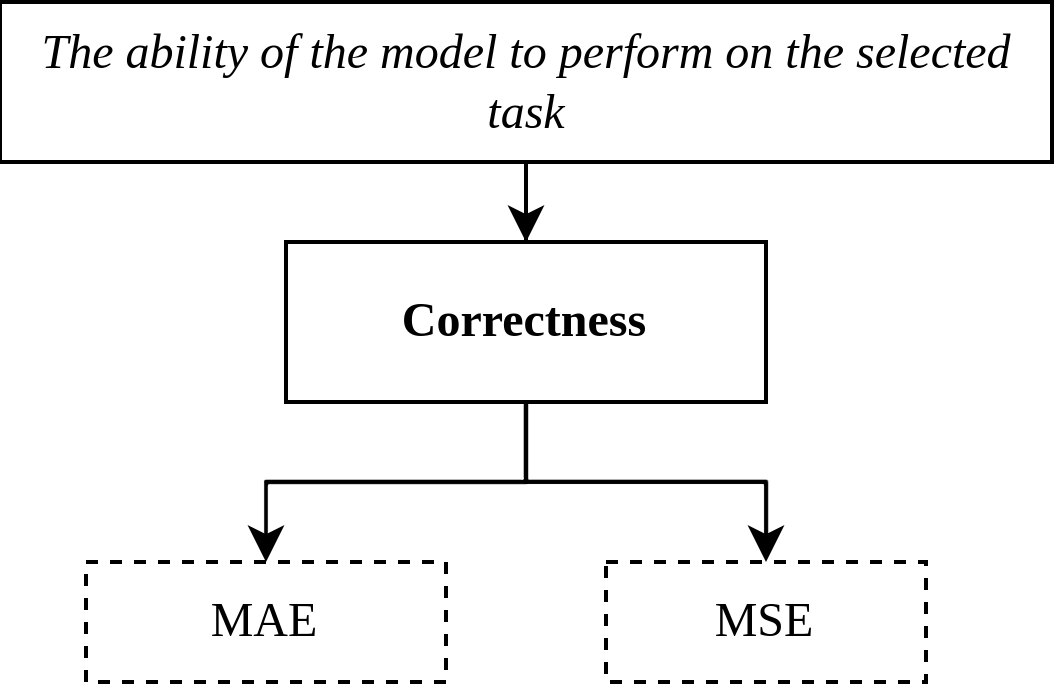
\includegraphics[width=0.6\textwidth]{goal_hierarchie_correctness}
%     \caption{Goal hierarchy: Correctness}
%     \label{fig:goal_hierarchie_correctness}
% \end{figure}

\subsection{Results}\label{subsec:results}

% Table wit hall used machine learning models and their metrics
\begin{table}[H]
    \begin{tcolorbox}[arc=0pt,boxrule=0.5pt]
        % \sisetup{group-minimum-digits = 4}
        \centering
        \begin{tabular}{llll}
            \toprule
            \thead{\textbf{Model Name}} & \thead{\textbf{MAE}}
            & \thead{\textbf{MSE}}
            & \thead{\textbf{RMSE}} \\
            \textbf{Random Forest}              & 0.16 & 0.04 & 0.21 \\
            \textbf{Random Forest (rand.split)} & 0.14 & 0.05 & 0.22 \\
            \hdashline
            \textbf{Support Vector Machine}     & 0.09 & 0.04 & 0.20 \\
            \textbf{SVM (rand. split)}          & 0.09 & 0.04 & 0.20 \\
            \bottomrule
        \end{tabular}
        \caption{Overview of the used machine learning models and their metrics.}
        \label{tab:ml_models}
    \end{tcolorbox}
\end{table}

\textit{Explanation of results...}


\section{Relevance}\label{sec:relevance}
% Does the model achieve a good bias-variance tradeoff? Which means neither overfitting or
% unterfitting the data.

% Bias variane trade-off
A model is considered relevant when it achieves a balance between bias and variance, avoiding
both overfitting and underfitting of the training data.
The relevance of the model can be quantified through the \textit{variance of cross-validation},
which proves insight into how the model perfoms when trained and evaluated on different subsets
of data and how generalizes.

% Explanation interpretation of variance
A low variance indicates that the model's performance is consistent across different folds,
suggesting that the model is not overfitting the training data.
Conversely, a high variance implies that the performance can vary significantly depending on the
specific data points used the test set, indicating a potential overfitting problem.

Figure~\ref{fig:variance-of-cv} shows how the variance of cross-validation was calculated.
The parameter $E$ denotes to the estimator which is used to calculate the \ac{CV} score.
The parameter $k$ denotes to the number of folds, which was set to 5 in this context.
As estimator for the trained models $R^2$ was used because this is usually the metric used to
evaluate the regression models.

\begin{figure}[h]
    \begin{tcolorbox}[arc=0pt,boxrule=0.5pt]
        \centering
        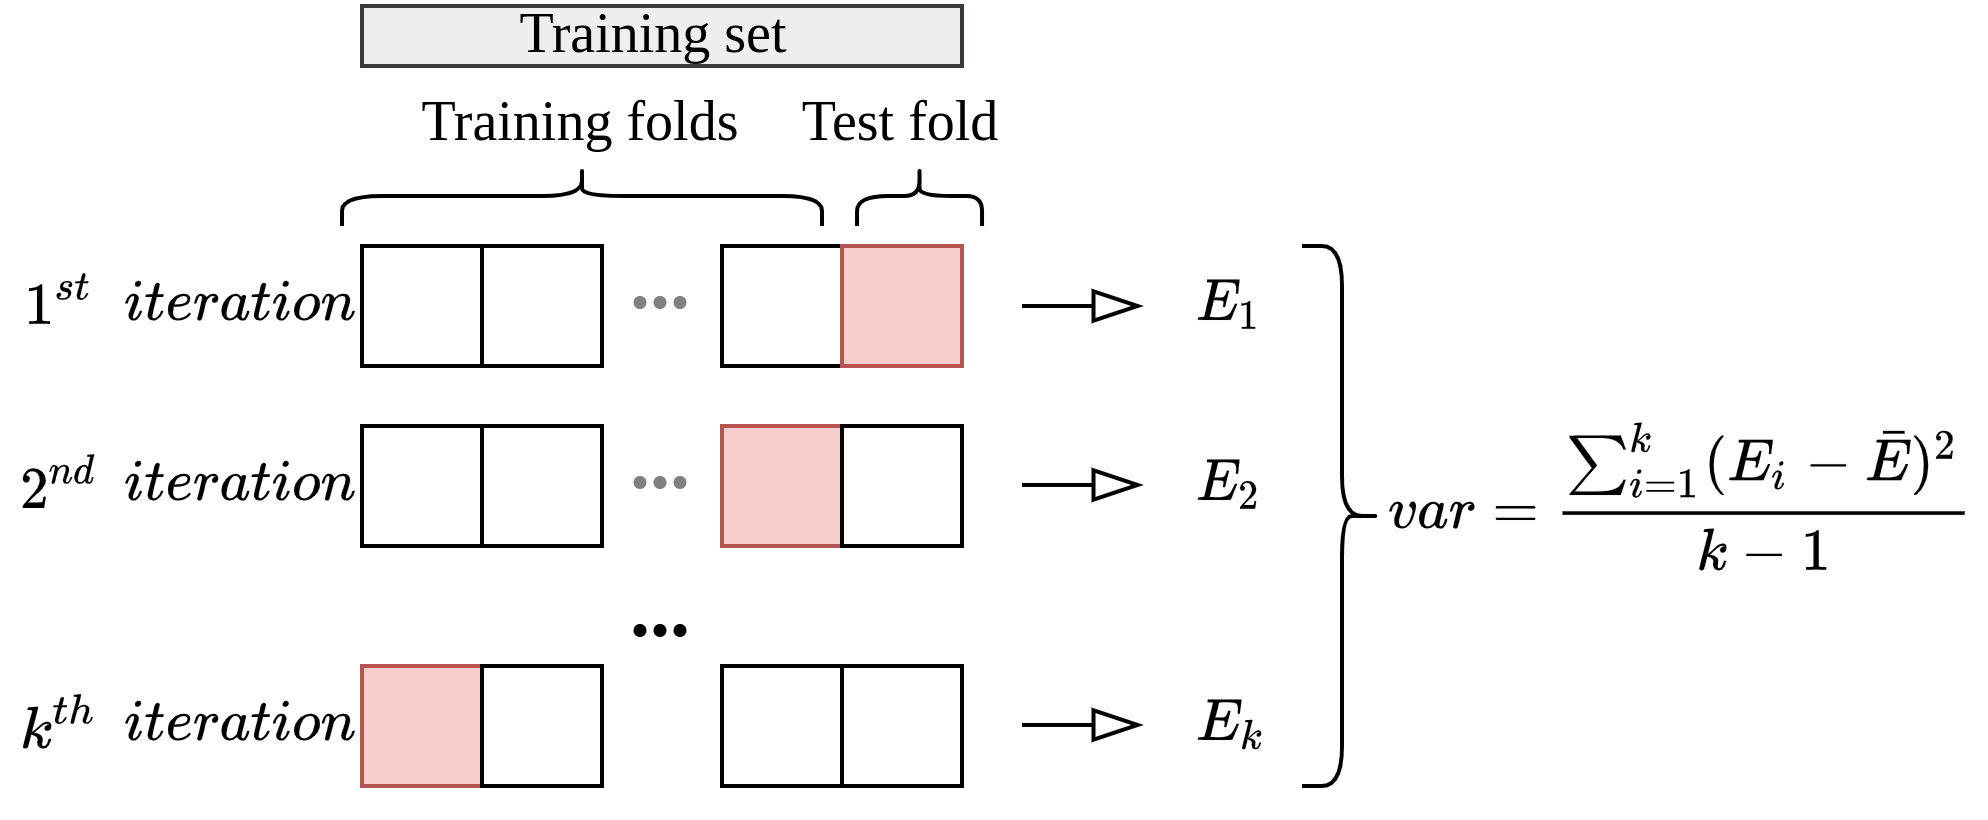
\includegraphics[trim=left botm right top, width=0.9\textwidth, clip]{variance_of_cv}
        \caption{Variance of cross-validation}
        \label{fig:variance-of-cv}
    \end{tcolorbox}
\end{figure}

For completeness the $R^2$ score is also shown int the table.
The $R^2$ is a statistical measure of how close the data are to the fitted regression line.
It returns a score between 0 and 1, where 0 means that the model does not explain any of the
variance in the response variable around its mean, and 1 means that the model explains all the
variance in the response variable around its mean.
Therefore, a high $R^2$ indicated a good model fir and good bias-variance tradeoff.
\cite[p. 43]{muller_introductionmachinelearning_2016}

\paragraph*{$R^2$}

\begin{equation}
    \label{eq:r2}
    R^2 = \frac{Explained\_variance}{Total\_variance\_targert\_variable}
\end{equation}

Table~\ref*{tab:ml_models_relevance} shows the variance of cross-validation and the $R^2$ for all
used machine learning models.
To calculate the variance of cross-validation the variance of Scikit-Learn's
\texttt{cross\_val\_score} was calculated.
Five-fold cross-validation was used to calculate the variance of cross-validation. The $R^2$ was
calculated with the formula~\ref{eq:r2}.

\begin{table}[H]
    \begin{tcolorbox}[arc=0pt,boxrule=0.5pt]
        % \sisetup{group-minimum-digits = 4}
        \centering
        \begin{tabular}{lll}
            \toprule
            \thead{\textbf{Model Name}} & \thead{\textbf{Variance of CV}}
            & \thead{\textbf{$R^2$}} \\
            \toprule
            \textbf{Random Forest}               & 0.034 & 0.771 \\
            \textbf{Random Forest (rand. split)} & 0.034 & 0.771 \\
            \hdashline
            \textbf{Support Vector Machine}      & 0.008 & 0.851 \\
            \textbf{SVM (rand. split)}           & 0.008 & 0.851 \\
            \bottomrule
        \end{tabular}
        \caption{Overview of the used machine learning models and their metrics.}
        \label{tab:ml_models_relevance}
    \end{tcolorbox}
\end{table}

\label{sec:robustness}


\section{Robustness}\label{sec:robustness2}
% Ability of the model to outliers, noise and other data quality issues
% Variance of cross-validation, fit

% Equalized Loss of Accuracy (ELA) 

% Definition of robustness
According to \cite{saez_evaluatingclassifierbehavior_2016} robustness "is the capability of an
algorithm to build models that are insensitive to data corruptions and suffer less from the
impact of noise" \cite[p. 2]{saez_evaluatingclassifierbehavior_2016}.
In this context the metric Equalized Loss of Accuracy (\ac{ELA}) was established to measure the
robustness of different machine learning models. But the \ac{ELA} is only usable for
classification models, therefore a different metric has to be found.

There are a number of ways to evaluate the performance of regression models, including mean
squared error (MSE), mean absolute error (MAE), and root mean squared error (RMSE). You can use
these measures to compare the performance of different regression models on a given task. Also
the $R^2$ can be used to measure the robustness of the model.

As mentioned in section~\ref{sec:dataset_exploration}~dataset~exploration the dataset has a high
quality with no outliers and no missing values.
Therefore, these data quality issues will be added to the dataset to measure the robustness of
the model.

\subsection{Missing values}
When applying the model to real-world data, there is a chance that some values are missing. Two
possible scenarios are possible:

\begin{enumerate}
    \item \textbf{Missing $Vt$-combinations}: There is no data available about a metal with a
    certain thickness and die opening. Reasons could be that the metal is not used in the
    industry or the data was never measured.
    \item \textbf{Missing values}: There is data for the $Vt$ combination but some values are
    missing because of general data quality issues.
    \item \textbf{Outliers}: There are values that are not in the range of the dataset. Reasons
    could be that the data was measured incorrectly.
\end{enumerate}

To measure all three of these scenarios, three different tests where created. The first test
measures the robustness of the model.

\subsubsection*{1. Missing $Vt$-combinations}
As can be seen Figure~\ref{fig:train_test_split} of the test and training dataset, all possible
$Vt$ combinations in the set parameter range where measured.
This is not the case in real-world data. Therefore, the robustness of the model has to be
measured with missing $Vt$ combinations.

Therefore, certain $Vt$ combinations were removed from the training dataset. The removed $Vt$
combinations were chosen randomly. The number of removed $Vt$ combinations was 10\% of the total
number of $Vt$ combinations in the training dataset.
Subsequently the model was trained on the training dataset with the removed data and evaluated on
the test dataset.
The performance of the mode is measures against the performance of the model trained with all data.

\subsubsection*{Calculation of the loss of accuracy}
The process described above was done 100 times, to mitigate the effect of the random selection of
the $Vt$ combinations.
The calculation of the loss of accuracy is follows Equation~\ref{eq:mla}, the metric is called
Mean Loss Of Accuracy (\ac{MLA}).

\paragraph*{Mean Loss Of Accuracy}
\begin{equation}
    \label{eq:mla}
    \text{MLA} = \frac{1}{100} \sum_{i=1}^{100} \left( \text{MSE}_{all} - \text{MSE}_{missing}
    \right)
\end{equation}

To calculate the loss off accuracy the models trained with missing $Vt$ combinations were
compared to the model trained with all data.
The difference between the \ac{MSE} of the models was calculated. The total loss of accuracy was
calculated by averaging the difference of the \ac{MSE} of the models.




\subsubsection*{2. Missing values}

\subsubsection*{3. Outliers and wrong data}
To measure the robustness of the model, outliers were added to the data. The outliers were added
to the data in the following way:

Outliers where added to the training dataset.
The model was trained on the training dataset.
The model was evaluated on the test dataset.
The outliers where removed from the training dataset.
The process was repeated 100 times.

\subsubsection*{Noise}
\textit{Not sure if I want to measure that.}


Note: This process of measuring the robustness of the model differs from the approach used by
\cite{siebert_constructionqualitymodel_} and \cite{saez_evaluatingclassifierbehavior_2016}.

\subsection{Results}

\begin{table}[H]
    \begin{tcolorbox}[arc=0pt,boxrule=0.5pt]
        % \sisetup{group-minimum-digits = 4}
        \centering
        \begin{tabular}{llll}
            \toprule
            \thead{\textbf{Model Name}} & {\thead{\textbf{Missing $Vt$-combinations} \\ \unit{loa}}}

            & {\thead{\textbf{Missing Values} \\ \unit{loa}}}
            & {\thead{\textbf{Outliers} \\ \unit{loa}}}          \\
            \toprule
            \textbf{Random Forest} & 0.034 & 0.000 & 0.771 \\
            \hdashline
            \textbf{Support Vector Machine} & 0.000 & 0.000 & 0.000 \\
            \bottomrule
        \end{tabular}
        \caption{Results of used machine learning models regarding the design principle robustness.}
        \label{tab:results_robustness}
    \end{tcolorbox}
\end{table}

\subsubsection*{\textit{Notes}}

\begin{itemize}
    \item \textit{An alternative metric instead of ELA could be the approach of Scher and Trügler
    . But it would be necessary to implement the metric in Python.}
    \item \textit{Decide if I want to evaluate noise as well or if the rest is enough.}
\end{itemize}


\section{Stability}\label{sec:stability}
% Does the artifact generate repeatable results when trained on different data?
% Leave-one-out cross-validation stability 
Stability is defined as the ability of the model to generate repeatable results when trained on
different data~\cite[p. 16]{siebert2022construction}.


One appropriate way to measure the stability of a model is to use \ac{LOOCV}, which is a
a form of \ac{CV} where one sample is used for validation and the remaining data is
used for training~\cite[p. 200--201]{gareth2013introduction}.

In order to evaluate the model the \ac{LOOCV} was repeated for all samples in the dataset
resulting in a total of $n$ iterations.
The stability of the model was determined by calculating the average prediction error across all
iterations, using the equation provided in Equation~\ref{eq:loocv} which is taken from~\cite[p.
201]{gareth2013introduction}.

\begin{tcolorbox}[arc=0pt,boxrule=0.5pt]
    \begin{equation}
        CV_{(n)} = \frac{1}{n} \sum_{i=1}^{n} \text{MSE}_{i}\label{eq:loocv}
    \end{equation}
\end{tcolorbox}

The approach provides an unbiased estimate of the model's generalization error
but this estimate is poor because only one samples is used for validation~\cite[p.
201]{gareth2013introduction}.

Therefore, it can not be used to make a statement about the generalization error of the model.
Since the goal is to measure repeatable results, the \ac{LOOCV} is a suitable metric to measure
the stability of the model.

%\textit{Which formula should I use?}
%
%\begin{tcolorbox}[arc=0pt,boxrule=0.5pt]
%    \begin{equation}
%        CV_{(n)} = \frac{\sum_{i=1}^{n} \text{MSE}_{i}}{1-n}\label{eq:loocv2}
%    \end{equation}
%\end{tcolorbox}

A low $CV_{(n)}$ value indicates a high stability of the model, because the model is able to
generate repeatable results when trained on different data.
Note: The method can be very time-consuming, especially for large datasets, but it may provide
more accurate estimates for small datasets.

%The stability the \ac{LOOCV} gives insights into the stability of the model. The stability is
%measured by calculating the variance of all \ac{CV} scores.

%\begin{tcolorbox}[arc=0pt,boxrule=0.5pt]
%    \begin{equation}
%        var_{(n)} = \frac{1}{n} \sum_{i=1}^{n} \left( \text{CV}_{(n)} - \text{CV}_{i} \right)^2
%        \label{eq:loocv_variance}
%    \end{equation}
%\end{tcolorbox}

%A low variance indicates that the model is stable which means that the model's performance is
%consistent across different training and testing sets.
%This is generally a desirable property for a model to have, as it suggest that the model ist not
%overfitting to the training data and is able to generalize well to unseen data.
%On the other hand, a high variances indicates an unstable model and is a sign of overfitting, as
%the model may be to closely tied to the training data and not generalize well to unseen data.

\subsection{Results}\label{subsec:results-stability}

\begin{table}[H]
    \begin{tcolorbox}[arc=0pt,boxrule=0.5pt]
        % \sisetup{group-minimum-digits = 4}
        \centering
        \begin{tabular}{ll}
            \toprule
            \thead{\textbf{Model Name}} & \thead{\textbf{$CV_{(n)}$}}
            \\
            \toprule
            \textbf{Random Forest}               & 0.053 \\
            \textbf{Random Forest (rand. split)} & 0.053 \\
            \hdashline
            \textbf{Support Vector Machine}      & 0.051 \\
            \textbf{SVM (rand. split)}           & 0.000 \\
            \bottomrule
        \end{tabular}
        \caption{Overview of the used machine learning models and their metrics.}
        \label{tab:results-stability}
    \end{tcolorbox}
\end{table}

\textit{Explanation of the results}


\section{Interpretability}\label{sec:interpretability}
% How well can the model be explained?
% Complexity measures (e.g., no. of parameters, depth)
Interpretability refers to the ease with which humans can understand and make sense of the
decisions made by a trained machine learning model~\cite[p. 16]{siebert2022construction}.
\cite{miller2019explanation} define interpretability as the "degree to which a human can
understand the cause of a decision"~\cite[p. 1]{miller2019explanation}.
Good interpretability is important because it allows users to trust and rely on the model, and it
can also help with debugging and improving the model (\textit{Source}).

Interpretable models will also deliver more insights for this project, as the goal is to
understand the relationship between the features and the target outcome.

When following the above definitions of interpretability, it is clear that it is not possible to
measure interpretability in a quantitative way.
No mathematical formula can be used to measure interpretability, but other methods can be used to
measure the interpretability of a model.
Interpretable models allow the usage of global model-agnostic evaluation methods which will be
used later in the evaluation of the models (see Section~\ref{sec:evaluation}).

In a first steps it has to be defined what makes a model interpretable.

\subsection*{Interpretable Models}
According to~\cite{molnar2020interpretable} one way to make a model interpretable is to limit the
choice of algorithms to those that produce interpretable results. Example of such
algorithms include linear regression, logistic regression and decision trees~\cite[p.
35]{molnar2020interpretable}.

\cite{molnar2020interpretable} defines three properties of interpretable models:

\textbf{Linearity} A linear model is one in which the relationship between features and the
target outcome is represented as a linear equation~\cite[]{molnar2020interpretable}.

\textbf{Monotonicity} A model with monotonicity constraints ensures that there is a consistent
relationship between a feature and the target out come across the entire range of the feature.
This can make it easier to understand the relationship.

\textbf{Interactions} Some models can automatically include
interactions between features to improve prediction, while other require manual creation of
interaction features.
However, too many or complex interactions can make the model more
difficult to interpret.

In the model selection for this thesis the focus is on interpretable models, as they are easier to
understand and explain, therefore mostly models are chosen which fulfill all three
properties.

Later in the thesis, the interpretability of the models is used to explain the results.

\subsubsection*{Big-O Notation}

Time complexity is a common way of measuring how fast or slow an algorith will perform for the
input size (Source). Usually the complextiy is measured with the big-O notation.
...

The term complexity is an overloaded term, normally complexity is measured with the big-O
notation and measures the scale in time as the number if inputs increases (Source).
However, in the context of machine learning, complexity is often used to refer to the
number of parameters in a model.

\subsubsection*{Number of Parameters}
More complex models tend to have more parameters and are therefore more difficult to interpret.
The number of parameters is calculated using the the \texttt{model.get\_params} function
in scikit-learn.

% EffiecientnetPaper?
Note: The Depth of the model could be used as well for the evaluation, but not all models have a
depth therefore this metric is not suitable.
The depths is representing the number of layers in the model.
A model with many layers, is generally more complex than a shallow network with fewer layers.

\subsubsection*{\textit{Notes}}

\begin{itemize}
    \item \textit{Space complecity -> How much memeory is needed?}
    \item \textit{Does using the big O notation make sense?}
\end{itemize}

\subsection{Results}\label{subsec:results2}

\begin{table}[H]
    \begin{tcolorbox}[arc=0pt,boxrule=0.5pt]
        % \sisetup{group-minimum-digits = 4}
        \centering
        \begin{tabular}{llll|ll}
            \toprule
            \thead{\textbf{Model Name}} & \textbf{\thead{Linear}} & \textbf{\thead{Monotone}} &
            \thead{\textbf{Interaction}}
            & \thead{\textbf{big-O}}
            & \thead{\textbf{Parameters}}
            \\
            \toprule
            \textbf{Decision Trees}      & No & Some & Yes & XX & XX \\
            \hdashline
            \textbf{Logistic Regression} & No & Yes  & No  & XX & XX \\
            \hdashline
            \textbf{SVM} & X & X  & XX & XX & 11 \\
            \hdashline
            \bottomrule
        \end{tabular}
        \caption{Overview of the used machine learning models and their metrics.}
        \label{tab:interpretable-models}
    \end{tcolorbox}
\end{table}

\subsubsection*{Notes}
\begin{itemize}
    \item \textit{Reasoning for results in table.}
\end{itemize}

\textit{Explanation of the results}


\section{Resource utilization}
% How much resources are required to train and run the model?
% Training time, runtime, storage space

To measure the resource utilization of the model, the following metrics are used:

% From Copilot
\paragraph*{Training time}
Measured in seconds. Refers to the time it takes to train the model.
Training a model requires resources such as memory, CPU, and GPU, therefore the longer it takes
to train a model, the more resources are required. According to resources utilization a shorter
training time is desirable.

The training time is measured using the \texttt{time.time} function in python. The function
returns the time in seconds since the epoch. The time is measured before and after the model is
fitted. The difference between the two times is the training time.

\paragraph*{Runtime}
Measured in milliseconds. It refers to the time it takes to make a prediction on data once it has
been trained.
It is an important measure not only for real-world application but also a faster runtime uses
less resources and is therefore more efficient.

\texit{Runtime = Inference time?}

\paragraph*{Inference time}
Measured in milliseconds. Time it takes to make a prediction.
A model that takes longer to make predictions may be more complex than a model that is able to
make predictions more quickly.


The runtime is measured using the \texttt{time.time}  function in python. On value is picked out
of the test set and the time is measured before and after the prediction is made. The difference
between the two times is the runtime.

\paragraph*{Storage space}
Measured in kilobytes. It refers to the amount of storage space required to store the model.
The more storage space required to store the model, the more resources are required to store it.
Therefore, a smaller storage space is desirable.
\begin{table}[H]
    \begin{tcolorbox}[arc=0pt,boxrule=0.5pt]
        % \sisetup{group-minimum-digits = 4}
        \centering
        \begin{tabular}{llll}
            \toprule
            \thead{\textbf{Model Name}} & {\thead{\textbf{Training time} \\ \unit[]{s}}}
            & {\thead{\textbf{Runtime} \\ \unit[]{ms}}} & {\thead{\textbf{Storage space} \\
            \unit{kb}}}
            \\
            \toprule
            \textbf{\ac{RF}}     & 0.0222  & 2.0275  & 80.2 \\
            \hdashline
            \textbf{LR}     & 0.000  & 0.000  & 0.000 \\
            \hdashline
            \textbf{SVM}     & 0.000  & 0.000  & 0.000 \\
            \bottomrule
        \end{tabular}
        \caption{Overview of the used machine learning models and their metrics.}
        \label{tab:ml_models_statbility}
    \end{tcolorbox}
\end{table}


\section{Interpretation Of Results}
Using the evaluation metrics described in the previous sections, the following results were
achieved...

\subsection*{Global Model-Agnostic Methods}
As already described in section~\ref{sec:interpretability}, only algorithms that are
interpretable where used for the evaluation.

\cite{molnar2020interpretable} differentiates between
model-specific and model-agnostic interpretability methods.
Model-specific methods are methods that are specific to a certain model type, for example,
decision trees.
Model-agnostic methods are methods that can be used with any model type, for
example, permutation importance.

Also \cite{molnar2020interpretable} differentiates between global and local interpretability. Global
interpretability refers to the ability to understand the overall behavior of the model, while
local interpretability refers to the ability to understand the behavior of the model for a
specific instance.

For the purpose of this thesis, the focus is on global model-agnostic methods, as they can be used
with any model type and provide an overview of the model's behavior.

\subsubsection*{Partial Dependence Plots}


\subsection*{Evaluation SVM (Only Notes)}
\cite[p. 104]{muller_introductionmachinelearning_2016}





